\chap{Modes: Pour ne pas toujours faire la même chose (avancé)}\label{ch.states}

Un programme VPL est composé d'une série de paires événement-action. Tous les événements sont vérifiés à tout moment et les actions appropriées sont effectuées. Ensuite, les événements sont vérifiés à nouveau, etc\ldots

Pour pouvoir programmer Thymio d'une façon un peu plus riche, il serait bien de pouvoir choisir quels événements sont à vérifier quand. Ainsi, il serait possible de créer des \textit{modes}. Thymio pourrait être en mode "recherche d'une ligne" ou en mode "suivi d'une ligne". Cela nous permettrait de programmer Thymio de deux façons différent en une seul fois. Gardons cet exemple de la ligne. Si Thymio perd de vue la ligne, il pourrait se mettre à parcourir la région dans laquelle il se trouve en évitant d'éventuels obstacles jusqu'à ce qu'il la retrouve. Dès lors, il se remettrait en mode "suivi de ligne" et continuerai son chemin. Cela permettrait d'avoir une assurance pour qu'en cas de problème Thymio se débrouille tout seul!

Pour jouer avec les modes, commencez par cliquer sur le symbole avancé du VPL:   \blk{advanced}.


\sect{Toc, toc}

Dans les programmes que nous avons réalisé jusqu'ici, nous avons souvent \emph{démarré} Thymio en appuyant sur un de ces boutons et \emph{arrêté} Thymio en appuyant sur un autre. Mais regardez votre ordinateur. Normalement, il n'a qu'un seul bouton pour l'allumer ou l'éteindre. Il serait possible de faire deux actions avec un seul bouton si Thymio pouvait se souvenir si vous avez déjà appuyé ou non sur son bouton.

\begin{bclogo}[couleur = pink!30, arrondi = 0.1, logo = \bccrayon, ombre = true]{Challenge!}Écrivez un programme en utilisant VPL qui fait que Thymio s'allume en rose si vous lui donnez une petite tape et qui fait que Thymio s'éteigne si vous lui donnez une autre tape.
\end{bclogo}

{\raggedleft \hfill Programme \bu{tap-on-off.aesl}}

Nous allons décrire ce programme en utilisant un \textit{diagramme d'états}, comme sur \cref{fig.turn-on-off}.

\begin{figure}
\begin{center}
\gr{diagramme_modes}{0.3}
\caption{Diagramme d'état, \textit{allumé - éteint}}\label{fig.turn-on-off}
\end{center}
\end{figure}

Le diagramme de \cref{fig.turn-on-off} comprend deux modes, \textit{allumé} et \textit{éteint}. Chaque mode peut-être atteint en suivant une flèche. Depuis le mode \textit{allumé}, il est possible de se rendre au mode \textit{éteint} en passant par une flèche \textit{Toc}. À l'inverse, depuis le mode \textit{éteint}, il est possible de se rendre au mode \textit{allumé}, en suivant l'autre flèche \textit{Toc}. Les flèches symbolisent les paires événement-action. Une tape qui fait s'allumer Thymio le fait passer du mode \textit{éteint} au mode \textit{allumé}.

Ce diagramme peut-être \textit{traduit} en français comme:

\begin{itemize}
	\item \textbf{Si} Thymio est  \textit{allumé} et qu'il reçoit une \underline{tape}, \textbf{alors} Thymio devient \textit{éteint}.
	\item \textbf{Si} Thymio est  \textit{éteint} et qu'il reçoit une \underline{tape}, \textbf{alors} Thymio devient \textit{allumé}.
\end{itemize}

Ainsi, nous pouvons voir qu'un même événement, une tape, peut induire deux actions différentes, en fonction du mode dans lequel se trouve Thymio au moment de la tape.

Le programme complet est donné sur \cref{fig.state-changing} . Nous allons maintenant le détailler.

\begin{figure}[h]
    \centering
    \subfigure[Une tape pour allumer ou éteindre]{ \label{fig.state-changing-a} 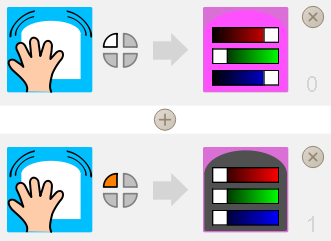
\includegraphics[width = 0.35\textwidth]{tap-on-off1}}
    \hspace{1cm}
    \subfigure[Une tape pour changer d'état]{ \label{fig.state-changing-b} 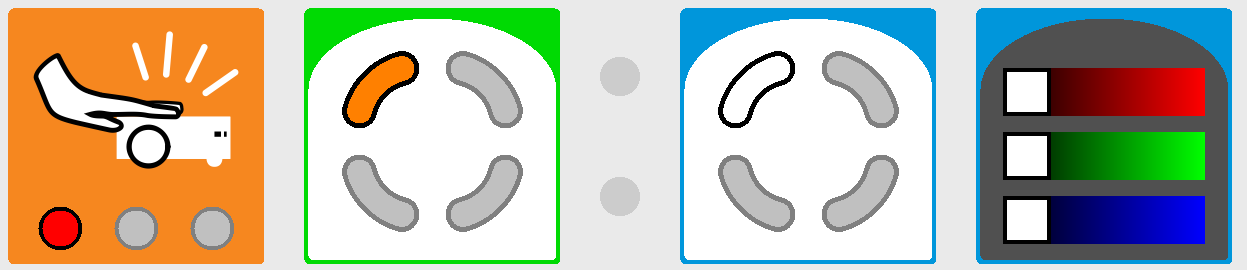
\includegraphics[width = 0.35\textwidth]{tap-on-off2}}
    \caption{Le programme complet avec deux types de paire événement-action}
    \label{fig.state-changing}
\end{figure}

Vous remarquerez le symbole \blk{states_icon} présent à côté de chaque événement. Ce symbole représente le mode dans lequel Thymio doit se trouver pour que l'action associée se déclenche. Chacune des quatre cases peut-être grise, blanche ou orange. Pour simplifier la suite du texte, nous allons numéroter les cases comme suit: \blk{states_icon_numbered}. Nous appelerons \textit{état}, la couleur d'une partie de ce cadran. Par exemple, Thymio pourra être en mode n$^\circ$1 si l'état de son cadran est [\textit{blanc, blanc, blanc, blanc}].

\begin{itemize}
	\item Une case \textbf{blanche} signifie \textit{état blanc}
	\item Une case \textbf{orange} signifie \textit{état orange}
	\item Une case \textbf{grise} signifie \textit{n'importe quel état}, \textit{blanc} ou \textit{orange}
\end{itemize}

Ainsi, sur \cref{fig.state-changing-a}, la première paire d'événement action est déclenchée si Thymio est en \textit{mode éteint} avec le cadran équivalent [\textit{blanc, gris, gris, gris}]. En suivant ce concept, la deuxième paire d'événement-action action est déclenchée seulement si Thymio est en \textit{mode allumé} avec le cadran équivalent [\textit{orange, gris, gris, gris}]. 

\begin{bclogo}[couleur = blue!30, arrondi = 0.1, logo = \bcinfo, ombre = true]{Truc et astuce!}C'est à vous de choisir les modes de Thymio et d'y associer un état du cadran. Nous aurions très bien pu associé le \textit{mode allumé} à l'état  [\textit{orange, blanc, blanc, orange}] et le \textit{mode éteint} à l'état [\textit{blanc, orange, blanc, orange}]. Il aurait simplement fallu rester cohérent dans tout le programme. Mais avouez que les états du cadran que nous avons choisi sont plus simple. Essayez toujours de rester le plus simple possible!
\end{bclogo}

Pour que le programme soit complet, il ne faut pas simplement avoir des lumières qui s'allument ou s'éteignent en fonction du mode de Thymio mais il faut aussi changer le mode de Thymio! C'est là que \cref{fig.state-changing-b} entre en jeu. La première paire événement-action signifie: \textit{Si Thymio reçoit une tape et qu'il est en \textbf{mode éteint}, alors passer en \textbf{mode allumé}}. De même, la deuxième paire événement action signifie: \textit{Si Thymio reçoit une tape et qu'il est en \textbf{mode allumé}, alors passer en \textbf{mode éteint}}.

Nous avons donc deux actions qui sont lancées lorsqu'un événement "tape" est détecté. Un changement d'état d'un cadran (donc un changement de mode) et un changement de lumière.

\sect{Combien de modes pour Thymio?}

Nous avons vu que le mode de Thymio est donné par l'état d'un cadran divisé en quatre parties. Chaque partie peut-être en état blanc, orange ou gris. Un état gris signifiant n'importe quel état, si un mode est associé à \blksm{states}, alors, si Thymio se trouve dans le mode \blk{states1} ou \blk{states2}, l'action associée à cette paire sera déclenchée. Une case grise n'est donc pas un état à proprement parlé.

Il y a \textbf{quatre cases} qui peuvent être dans \textbf{deux états} différents. Les mathématiques nous disent donc qu'il peut y avoir $4^2 = 16$ modes! Ils sont tous illustrés sur \cref{fig.every-states}.

\begin{figure}[h]
    \centering
    \subfigure[Tous les états possibles de Thymio]{\label{fig.every-states} \includegraphics[width = 0.35\textwidth]{all_states}} 
    \hspace{1cm}
    \subfigure[La lumière indique le mode de Thymio]{\label{fig.state-leds} 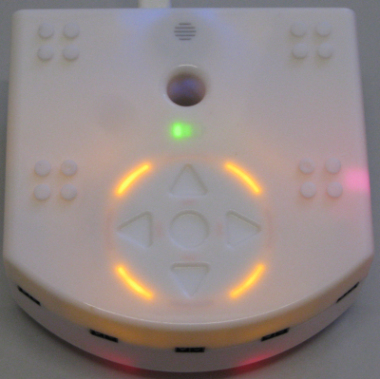
\includegraphics[width = 0.35\textwidth]{state-leds}}
    \caption{Les états de Thymio et leur représentation}
\end{figure}

Le mode de Thymio est physiquement illustré par des arcs de cercles lumineux. Le mode blanc éteint l'arc de cercle correspondant alors que le mode orange l'allume. \Cref{fig.state-leds} montre l'état complètement orange de Thymio.

\sect{Tête chercheuse}

\begin{bclogo}[couleur = pink!30, arrondi = 0.1, logo = \bccrayon, ombre = true]{Challenge!}Écrivez un programme en utilisant VPL qui fait que Thymio tourne sur lui-même, dans le sens inverse des aiguilles d'une montre, à la recherche d'un objet. Lorsqu'il le repère avec son capteur tout à droite, Thymio doit tourner dans l'autre sens et s'aligner sur l'objet.
\end{bclogo}

{\raggedleft \hfill Programme \bu{tete-chercheuse.aesl}}

Comme il est aisé de représenter ce challenge avec un diagramme d'état, nous le donnons sur \cref{fig.State_diagram_mouse}.

\begin{figure}[h]
\begin{center}
\gr{State_diagram_mouse}{0.4}
\caption{Diagramme d'état}\label{fig.State_diagram_mouse}
\end{center}
\end{figure}

Pour réaliser ce programme, nous avons besoin de trois modes. 

\begin{itemize}
	\item Le \textbf{premier mode} est l'\textbf{arrêt}. Thymio est arrêté, il attend qu'on appuie sur son bouton central pour lancer la recherche. L'état du cadran associé à ce mode est 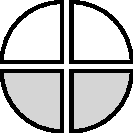
\includegraphics[scale=0.3]{Mode1}
	\item Le \textbf{deuxième mode} est la \textbf{recherche}. Thymio cherche l'objet en tournant sur lui-même. Il ne sortira de ce mode que lorsqu'il verra l'objet sur son capteur tout à droite. L'état du cadran associé à ce mode est 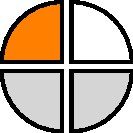
\includegraphics[scale=0.3]{Mode2}
	\item Le \textbf{troisième mode} est l'\textbf{alignement}. Thymio tourne dans l'autre sens pour s'aligner avec l'objet. Il ne sortira de ce mode que lorsqu'il verra l'objet en face de lui. L'état du cadran associé à ce mode est 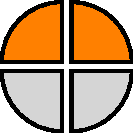
\includegraphics[scale=0.3]{Mode3}
\end{itemize}

En regardant les flèches et les indications de \cref{fig.State_diagram_mouse}, nous pouvons voir que:

\begin{itemize}
	\item Pour passer du mode 1 au mode 2, nous devons appuyer sur le bouton central de Thymio
	\item Pour passer du mode 2 au mode 3, Thymio doit trouver l'objet avec son capteur tout à droite
	\item Pour passer du mode 3 au mode 1, Thymio doit trouver l'objet avec son capteur central, il doit donc être aligné avec l'objet.
\end{itemize}

En suivant toutes ces indications, nous pouvons construire le programme illustré sur \cref{fig.prog_tete_chercheuse}.

\begin{figure}[h]
    \centering
    \subfigure[]{\includegraphics[width = 0.35\textwidth]{prog_tete_chercheuse1}} 
    \hspace{1cm}
    \subfigure[]{\includegraphics[width = 0.35\textwidth]{prog_tete_chercheuse2}}
    \caption{Thymio tête chercheuse}
    \label{fig.prog_tete_chercheuse}
\end{figure}

\begin{bclogo}[couleur = pink!30, arrondi = 0.1, logo = \bccrayon, ombre = true]{Challenge!}Écrivez un programme en utilisant VPL qui fait que Thymio suive une ligne en étant bleu et, s'il la perd, qu'il devienne rouge et la recherche à gauche et à droite jusqu'à ce qu'il la retrouve.
\end{bclogo}